
C++的标准化过程很民主,委员会称为WG21(21工作组),成立于1990-1991年。21工作小组的成员如下:

\begin{itemize}
\item 
召集人:主持WG21会议,制定会议日程,并任命研究小组

\item 
项目编辑:对C++标准的草案进行修改

\item 
秘书:对WG21会议进行记录
\end{itemize}

该图展示了委员会的各个子小组和研究小组。

\begin{center}
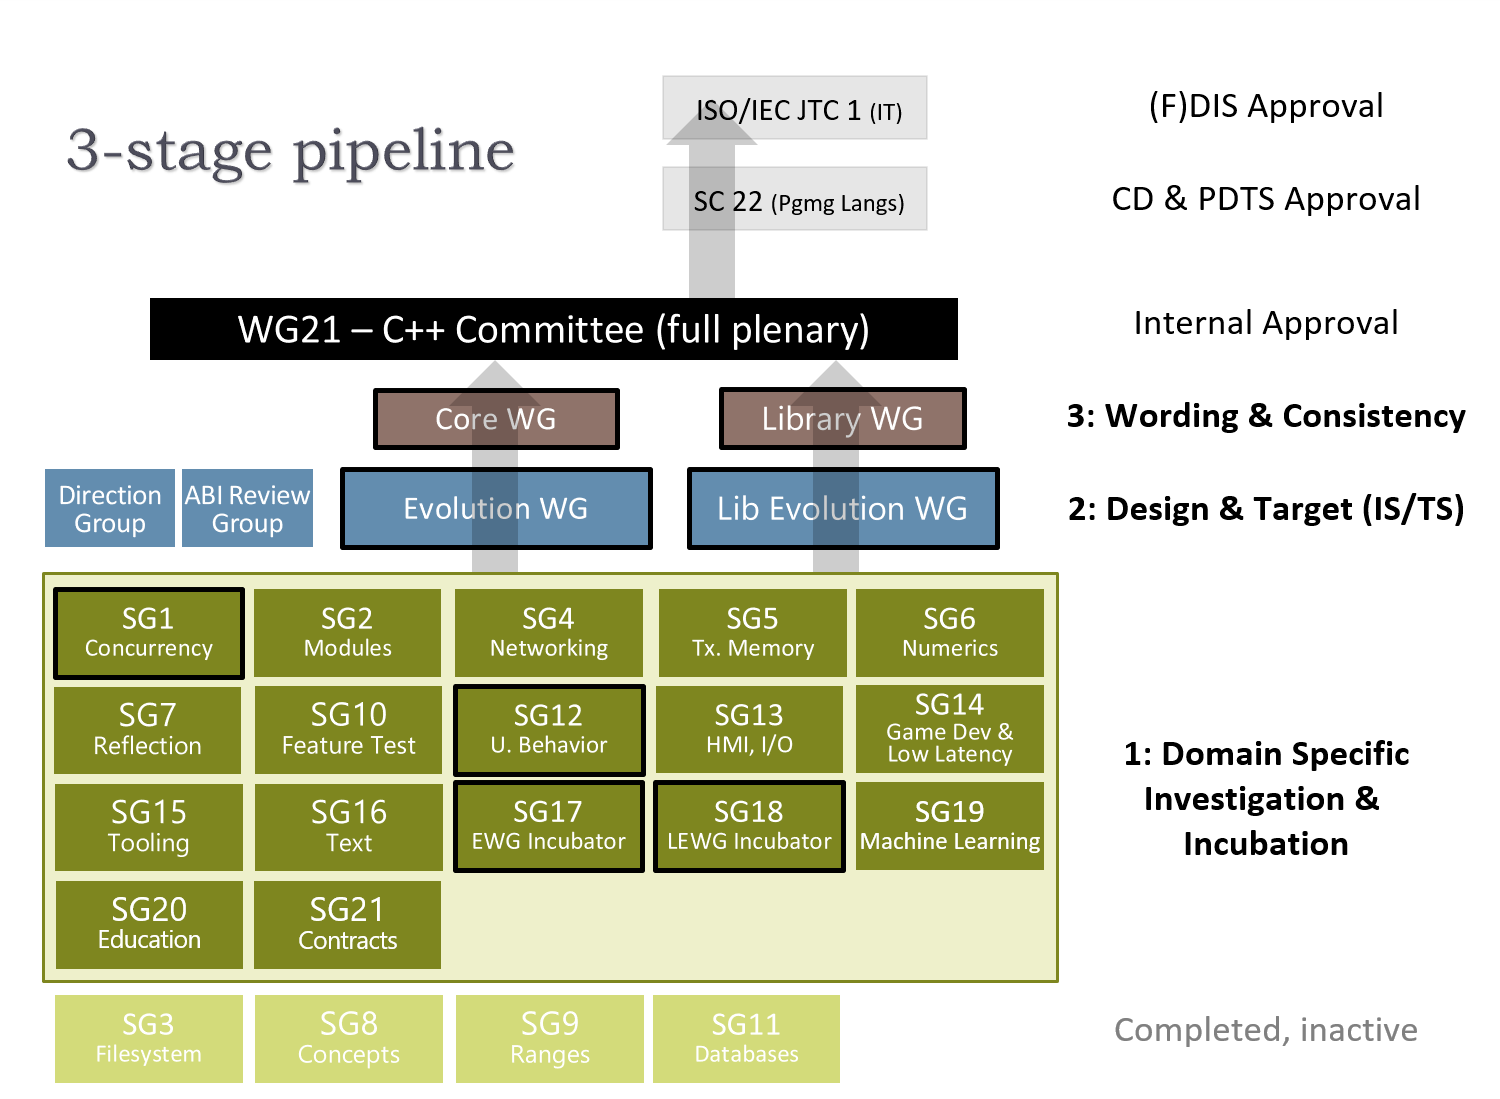
\includegraphics[width=0.8\textwidth]{content/1/chapter2/images/1.png}\\
研究小组在C++标准化过程中组成情况
\end{center}

委员会分为三个阶段,由几个小组组成。SG代表研究组(Study Group)。